\documentclass[openany,oneside]{book}

\usepackage{amsmath}
\usepackage{amssymb}
\usepackage{cag}
\usepackage{fancyhdr}
\usepackage{float}
\usepackage{geometry}
\usepackage{graphicx}
\usepackage{epstopdf}
\usepackage{listings}
\usepackage{microtype}
\usepackage{nag}
\usepackage{titlepic}
\usepackage[usenames,dvipsnames,svgnames,table]{xcolor}

%\usepackage{arevmath}
\usepackage{lmodern}
\usepackage{bera}

\usepackage{hyperref}

\pagestyle{fancy}

%\geometry{a4paper} % May funkify floating listings

\definecolor{TUBlue}{RGB}{61,152,222}
\definecolor{SpartanGreen}{RGB}{24,69,59}


\hypersetup{
    colorlinks=true,
    citecolor=Blue,
    linkcolor=Blue,
    urlcolor=Green
}

\lstset{
  language=fortran,
  basicstyle=\ttfamily,
  commentstyle=\itshape\color{Blue},
  keywordstyle=\bfseries\color{DarkRed},
  stringstyle=\color{Magenta},
  columns=fixed,
  numbers=left,
  numberstyle=\footnotesize\color{lightgray},
  numberblanklines=true,
  showstringspaces=false,
  caption=\lstname,
  firstnumber=auto,
  frame=single,
  rulesepcolor=\color{black},
  gobble=2 % Allow indentation in LaTeX source for readibility
}

\lstdefinestyle{prompt}{
  language=bash,
  caption=,
  commentstyle=\itshape\color{gray},
  keywordstyle=\ttfamily,
  numbers=none,
  frame=none
}

\newcommand{\keyword}[1]{\texttt{\bfseries\color{DarkRed}#1}}
\newcommand{\str}[1]{\texttt{\color{Magenta}#1}}
\newcommand{\Chapter}[2]{\chapter[#1]{#1\\[1ex]\Large#2}} 

\renewenvironment{quote}{\list{}{\leftmargin=8\parindent}\item\relax}{\endlist}

%\widowpenalty=3000
%\clubpenalty=3000

\begin{document}

\title{ICCP Coding Manual}
\author{Connor Glosser, Jos Seldenthuis, Chris Verzijl, \\ 
  Erin McGarrity, and Jos Thijssen}
  \titlepic{
    \begin{figure}[b]
      \centering
      
\includegraphics[width=0.33\pdfpagewidth]{figures/MSU_logo.pdf} \hfill
      
\includegraphics[width=0.33\pdfpagewidth]{figures/TU_logo.pdf}
    \end{figure}
  }

\frontmatter
\maketitle

\newpage
\null
\vfill
\begin{center}
  \includegraphics[width=0.15\textwidth]{figures/by-nc-sa.eps}
\end{center}
This work, including its figures and \LaTeX\ source code, is licensed under the Creative Commons Attribution-NonCommercial-ShareAlike 4.0 International License. 
To view a copy of this license, visit \url{http://creativecommons.org/licenses/by-nc-sa/4.0/deed.en_US}.

\tableofcontents
%\lstlistoflistings

\Chapter{Introduction}{}
\label{chap:Introduction}

\begin{quote}\small
\emph{``There are only two kinds of programming languages: \\ those people always bitch about and those nobody uses.''} \\ \hspace*{\fill}---Bjarne Stroustrup
\end{quote}
These coding notes are a short introduction to scientific programming, combined with a list of best practices.
Programming is an art; it takes time to become experienced, but these guidelines will help you to avoid common mistakes.
Follow them! They were born out of years of experience, and will save you and your instructors a lot of time.
You will be spending most of your time thinking about your algorithms and debugging your code, not actually writing it.
Writing clean code, following best practices, and not trying to be overly clever will make your life a lot easier.

Choosing a programming language is about picking the right tool for the job.
In the case of ICCP, that means Fortran.
We won't force you to use a particular language, but for most of the programs you'll write, dynamic languages such as MATLAB or Python are too slow, while C, \Cplusplus, and Java lack the built-in numerical facilities\footnote{It's called Fortran---FORmula TRANslation---for a reason!} (with Java also being slow).
Fortran is over half a century old---it first appeared in 1957---and can be a bit quirky, but for better or worse, it's still the industry standard when it comes to scientific computing.
Besides, modern Fortran---the most recent standard updates appeared in 2003 and 2008---is not nearly the monstrosity it used to be; it's actually a quite pleasant language for computational physics.
Even if you already have some experience with another language, take it from us that both you and your code will be faster if you use Fortran for ICCP.
If you want to continue in computational physics you'll encounter it sooner or later anyway (think LAPACK), and ICCP is the perfect time to learn.

These notes are by no means a Fortran reference.
High-quality documentation can be easily found online.
Good starting points are \url{http://fortran90.org} and \url{http://en.wikipedia.org/wiki/Fortran_language_features}.
The \emph{Intel Fortran Compiler Language Reference} is freely available (Google it).
We also recommend \emph{Modern Fortran Explained} by Metcalf, Reid and Cohen, or \emph{Fortran 95/2003 for Scientists \& Engineers} by Chapman.

Finally, you can find an up-to-date version of all the examples shown here (as well as useful helper modules and visualizations) at \url{https://Github.com/cglosser/libICCP}.
See the \nameref{chap:Revision control} chapter for details on cloning the code from Github.

\mainmatter
\Chapter{Getting your toes wet}{with Fortran and Linux}
\label{chap:Getting your toes wet}
\begin{quote}\small
  \emph{``1957: John Backus and IBM create FORTRAN\@. There's nothing funny about IBM or FORTRAN\@. It is a syntax error to write FORTRAN while not wearing a blue tie.''} \\ \hspace*{\fill}---James Iry
\end{quote}

For this course we recommend using the GNU Fortran compiler, as it is free and of reasonably high quality.\footnote{You're welcome to use the Intel Fortran compiler, which is free on Linux, but remember to change the compiler flags, since they differ from \texttt{gfortran}.}
Linux is the platform of choice, since it's most suited to programming and high-performance computing.\footnote{As of this writing, 476 of the \href{http://www.top500.org/list/2013/11/}{TOP500} supercomputers in the world run some form of Linux.}
OS~X, being a Unix variant, is also an option, but installing the required packages is generally a bit more work.
In these notes we will assume that you're using Ubuntu.\footnote{You can use Ubuntu as a native installation, run it from a flash drive, under a virtual machine, or under Windows using Wubi.
Ask your instructor.}

After booting Ubuntu, you need to install a Fortran compiler.
Open a terminal and at the prompt (the \$) type
\begin{lstlisting}[style=prompt, nolol]
  $ sudo apt-get install gfortran gfortran-doc
\end{lstlisting}
\emph{Note that anything you type in the console is case-sensitive!}
This command grants the package manager (\texttt{aptitude}) privileges to search for and then install the \texttt{gfortran} package and its documentation.
You may also find it useful to install the \LaTeX\ typesetting system for writing reports.
You can install it with another call to \texttt{apt-get}:
\begin{lstlisting}[style=prompt, nolol, breaklines=false]
  $ sudo apt-get install texlive # or texlive-full for a complete installation
\end{lstlisting}

Once you have \texttt{gfortran} installed, you can start writing programs.
You will generally compile and run your programs from a terminal window (also called a \emph{console}).
A few useful commands include:
\begin{lstlisting}[style=prompt, nolol, linewidth=30cm]
  $ ls           # display the contents of the current directory
  $ ls -l        # display contents with extra details
  $ cp file path # copy `file' to `path'
  $ mv file path # move `file' to `path'
  $ rm file      # remove `file'
  $ mkdir dir    # create a new directory called `dir'
  $ cd dir       # change current directory to `dir'
  $ rmdir dir    # remove directory `dir' (only if it's empty)
  $ rm -r dir    # remove directory `dir' (even if it's not empty)
  $ man cmd      # provide documentation on `cmd'
\end{lstlisting}

For your first program, open a terminal, create a directory for ICCP files and open your first Fortran file by typing
\marginnote[-0.5cm]{Modern shells all have a feature called
  \emph{tab completion}\index{Tab completion}; hit the \texttt{TAB} key after you've entered part of a command and the shell will attempt to fill in the rest of the command for you.}
\begin{lstlisting}[style=prompt, nolol, linewidth=30cm]
  $ mkdir iccp          # create a new directory called 'iccp'
  $ cd iccp             # move to the new directory
  $ gedit myprog.f90    # open a text editor with the file 'myprog.f90'
\end{lstlisting}
The gedit text editor pops open in which you can type the program in \cref{lst:myProg}.
You can probably guess what this program does, however, a few remarks are in order:
\begin{itemize}
  \item The program starts with a declaration of variables.\index{Fortran!types}
    \texttt{\keyword{real}(8)} denotes a floating-point variable with double (8 byte) precision.
    Similarly, \keyword{integer} denotes an integer number.\footnote{Fortran intrinsic types include \keyword{logical}, \keyword{integer}, \keyword{real}, \keyword{complex}, and \keyword{character} data. Modern Fortran also gives you the ability to define your own datatypes.}
    Not specifying a size generally defaults to 4-byte precision.
    \keyword{implicit none}\index{Fortran!implicit none@\keyword{implicit none}} prevents Fortran from trying to infer the type from the variable name, which is a major source of bugs---\emph{always include this!}
  \item The attribute \keyword{parameter}\index{Fortran!parameter@\keyword{parameter}} specifies that we are declaring a constant.
    Although Fortran is case-insensitive, it is considered good practice to always use uppercase names for constant variables.
  \item Note the calculation of $\pi$ as \texttt{4*\keyword{atan}(1d0)}---convenient and accurate.
  \item Single-precision (4 byte) floating-point numbers can be written as \texttt{0.1} or \texttt{1e-1} (scientific notation).
    For double-precision numbers, use \texttt{d} instead of \texttt{e} in scientific notation, \eg, \texttt{1d-1}.
    It is also possible to specify the precision as a suffix: \texttt{1.0\_4} for single and \texttt{1.0\_8} for double precision.
    This also works for integers.
  \item \texttt{\keyword{integer} :: fibonacci(N)} allocates an array of 20 integers, with the array\index{Fortran!arrays} index\footnote{Array indices can start at any integer by replacing \texttt{N} with a lower and upper bound separated with a colon. Thus, \lstinline$real :: myArray(-312:74)$ means \texttt{myArray} starts at index -312 and runs through index 74.} running from 1 to 20.
  \item `\texttt{*}' is multiplication, `\texttt{**}' is exponentiation.
  \item The \keyword{print} statement on line 24 contains the format code\index{Fortran!format codes} \str{"(4I6)"}.
    This tells Fortran to print 4 records of integer type, each having a width of 6 characters (including spaces), per line. 
    \Cref{tbl:format codes} gives the format codes for other intrinsic types.
    \begin{margintable}
      \begin{tabular}{ll}
        \toprule
        Format string & Meaning \\
        \midrule
        \texttt{Iw}    & integer \\
        \texttt{Ew.d}  & real  (decimal form)\\
        \texttt{ESw.d} & real  (scientific form)\\
        \texttt{ENw.d} & real  (engineering form)\\
        \texttt{Lw}    & logical \\
        \texttt{A}     & character data\\
        \bottomrule
      \end{tabular}
      \caption{\label{tbl:format codes}Format codes for intrinsic types. \texttt{w} gives the width of a record, and \texttt{d} gives the number of places to the right of the decimal.}
    \end{margintable} 
  \item Comments in Fortran start with `\texttt{!}' and last until the end of the line.
  \item Dividing integers \textcolor{red}{\textbf{results in an integer}}\index{Fortran!integer division}, so \texttt{3 / 2 == 1} instead of 1.5 as you might expect.
    Multiplying by \texttt{1d0} on line 28 forces Fortran to do a double-precision floating-point calculation.
\end{itemize}
Now we compile and run the program.
Compiling means translating the Fortran source code into machine code (processor instructions).
This can be done by simply typing
\begin{verbatim}
$ gfortran myprog.f90
\end{verbatim}
which will result in the executable file \texttt{a.out}.
This is the default name for the output.
You can specify a different name by compiling with
\begin{verbatim}
$ gfortran myprog.f90 -o myprog
\end{verbatim}
which results in a program with the name \texttt{myprog}.
During compilation, the compiler may generate error messages and warnings.
The errors must be fixed before an actual running program is produced, and it is good practice to also make sure no warnings are generated.

The compilation process can be tuned by passing certain command-line arguments to the compiler.
We recommend using always at least the following:
\begin{verbatim}
$ gfortran -Wall -Wextra -march=native -O3 myprog.f90 -o myprog
\end{verbatim}
\begin{itemize}
  \item \texttt{-Wall}\index{compiler flags!-Wall} and \texttt{-Wextra}\index{compiler flags!-Wextra} turn on all warnings.
    This may generate a lot of messages, but fixing them all leads to much cleaner code.
    This can be a huge time saver; not only for you, but also for your instructors!
    If your program doesn't behave as expected, first try to fix all warnings before asking your instructors for help.
  \item \texttt{-march=native}\index{compiler flags!-march=native} tells the compiler to generate machine code using all available processor instructions on your machine. 
    On modern CPUs this leads to much faster code, since \texttt{gfortran} can use vector instructions.
    The downside is that it can result in executables that will not run on a different machine.
  \item \texttt{-O3}\index{compiler flags!-O3} turns on all optimizations.
    This increases the compilation time significantly, although it should still be fast enough for the programs you'll write in ICCP.
    The run time of your program, on the other hand, will dramatically decrease.
    The only reason not to use this flag is that it might interfere with the debugger (see below).
  \item A possible additional optimization flag is \texttt{-ffast-math}\index{compiler flags!-ffast-math}.
    This flag enables floating-point optimizations which might reduce accuracy or result in incorrect behavior, especially in situations such as divide-by-zero.
    We therefore recommend not using this flag until you have verified that your program produces the correct results.
    After that you can use it to make your program faster, but do check that it still behaves correctly.
  \item Finally, if your code starts throwing segmentation faults (segfaults), consider using the \texttt{-fbounds-check}\index{compiler flags!-fbounds-check}\index{segmentation fault} flag.
    Segfaults usually occur because you've run an index off the end of an array, so compiling with this flag turns on runtime bounds checking (at the expense of significantly reduced performance).
\end{itemize}
If the program compiled correctly, you can run it by typing \texttt{./a.out} or \texttt{./myprog}.
Note that \texttt{./} specifies the \emph{path}, \ie, the location where to find the program.
The dot means the current directory (similarly, \texttt{..} refers to the parent directory), and the slash separates directories and file names (like the backslash in DOS and Windows).

\lstinputlisting[float=h!,label=lst:myProg]{examples/myProg.f90}

\Chapter{Structuring your code}{(to keep your instructors sane!)}
\label{chap:Structure}

\begin{quote}\small
  \emph{``Always code as if the guy who ends up maintaining your code will be a violent psychopath who knows where you live.''} \\ \ldots because that guy might be you in six months. \\ \hspace*{\fill}---Martin Golding
\end{quote}
Readability is the most important quality of your code.
It's more important even than being bug-free; you can fix a readable but incorrect program, while an unreadable program is next to useless even if it works.
As an example of what not to do, take a look at the gem in \autoref{lst:snppic}.
\lstinputlisting[float=htb,label=lst:snppic]{examples/snppic.f}
Originally written in FORTRAN IV for an IBM 1130 (in 1969!), it is a perfect example of spaghetti code and it makes me want to pick out my eyes with a fondue fork.
If you can figure out what it does, I'll buy you a beer.\footnote{It's part of one of the first open source programs in history, so no snooping with Google!}

To keep your code readable, you need to structure your program in a smart way while following a reasonable coding style.
A coding style encompasses things like naming conventions, indentation, comment rules, \emph{etc.}; see the \nameref{chap:Coding style}~chapter below for our recommendations.
In this chapter we focus on structure.

\section{Functions and subroutines}

As a (silly) example, let's say you need to sum all integers in a certain interval.
Programmers are lazy, so we're going to write a program to do that for us.
Gauss, of course, found a way to do this very quickly, but for the sake of the example, let's pretend we don't know about it and use \autoref{lst:SumsBeforeGauss} instead.
\lstinputlisting[float=htbp,label=lst:SumsBeforeGauss]{examples/SumsBeforeGauss.f90}
Note that we can't use the word \texttt{sum} as a variable name, since that's a Fortran intrinsic\footnote{Fortran \emph{occasionally} uses reserved keywords in multiple ways, such as \keyword{dim} (the two-argument function) and \texttt{dim} (an argument to several array-based subroutines), though the meaning is usually clear.}, so we use \texttt{total} instead.
This program is simple, clean, and doesn't need comments to show what it does.
However, we can do better.
Summing numbers in an interval is a generic mathematical operation, which we might need to do more often.
It therefore makes sense to move that code to a separate subroutine which we only have to write once and can then reuse as many times as we need.
We can do this in Fortran, with the subroutine seen in \autoref{lst:SumsBeforeGauss_subroutine}.
\lstinputlisting[float=htbp,label=lst:SumsBeforeGauss_subroutine]{examples/SumsBeforeGauss_subroutine.f90}
Fortran subroutines are invoked with the keyword \keyword{call} followed by the name of the routine and an optional list of parameters in parentheses.
The code for the subroutine itself appears after the keyword \keyword{contains}.
We don't have to type \keyword{implicit none} again, since that's inherited from the program.
When declaring the parameters, we need to specify not only the type, but also how we're going to use them, \ie, the \emph{intent}.\index{Fortran!intent(in/out)@\keyword{intent (in}/\keyword{out)}}
For input and output parameters, we use \texttt{\keyword{intent}(\keyword{in})} and \texttt{\keyword{intent}(\keyword{out})}, respectively.
For parameters functioning as both, we use \texttt{\keyword{intent}(\keyword{inout})}.

\texttt{stupid\_sum} is essentially just a mathematical function.
Wouldn't it then be nice to be able to use it that way, by simply invoking it with \texttt{total = stupid\_sum(first, last)}?
Fortunately, \autoref{lst:SumsBeforeGauss_function} demonstrates a way to do just that.
\lstinputlisting[float=htbp,label=lst:SumsBeforeGauss_function]{examples/SumsBeforeGauss_function.f90}
A function in Fortran is just a subroutine returning a value.
We therefore need to specify the type of (the result of) the function as well as its arguments.
This type is given before the keyword \keyword{function}.
\texttt{\keyword{result}(total)} tells Fortran that the local variable \texttt{total} (of type \keyword{integer}) holds the return value of the function.

Splitting reusable code off into subroutines and functions is absolutely necessary for any non-trivial program.
Always take the time to think about the structure of your program before you start typing.
The golden rule here is: \emph{every function or subroutine should do one thing and do it well.}
In practice this also means they should be small; if your function doesn't fit on a single screen, that's usually an indication that you should split it up.
Besides making the code more readable, this also makes it easier to modify.
Let's say that you suddenly discover Gauss' trick for summing intervals.
All you need to do then is replace \texttt{stupid\_sum} by \texttt{smart\_sum} (\autoref{lst:smart_sum_function}).
\lstinputlisting[float=t!,label=lst:smart_sum_function]{examples/smart_sum_function.f90}
You don't have to search through all your code to change the calculation everywhere; you just update the function and your entire program suddenly becomes a lot faster.

\section{Modules}

Many functions and subroutines are reusable not only within a single program, but also between programs.
In that case it is a good idea to place those routines in a module.\footnote{Some subroutines---particularly those that allocate arrays that appear as arguments---require you to write an explicit interface for them \emph{or} place them within a module (so the compiler can generate the interface for you).}
For example, if you envisage using Gauss' algorithm very often in the future, you might want to create the module \texttt{gauss.f90} given in \autoref{lst:gauss}.
\lstinputlisting[float=htbp,label=lst:gauss]{examples/gauss.f90}
By default, all functions and subroutines in a module are visible to external programs.
This can cause collisions with similarly names functions in other modules, especially in the case of helper routines that are only used within the module.
Common practice is therefore to specify the \keyword{private} keyword to change the default behavior; only the routines that are explicitly made public are then usable elsewhere.

Any program can now use the functions in \texttt{gauss.f90} by simply specifying \texttt{\keyword{use} Gauss} (\autoref{lst:Sums}).
\lstinputlisting[float=htbp,label=lst:Sums]{examples/Sums.f90}
You now have two different files that need to be compiled to produce a working program.
It's possible to do this by hand, but there is a much easier way with \nameref{chap:Makefiles}.


\Chapter{The magic of Makefiles}{}
\label{chap:Makefiles}

Once your programs become larger, it is convenient to split the source code into several files.
However, to obtain a running program, each of these files has to be compiled separately (resulting in a \emph{relocatable object file}, with extension \texttt{.o}) and then combined (linked) into a single program.
Doing this by hand quickly becomes tedious, so we resort to using Makefiles.
We create a file called \texttt{Makefile} that contains all compiler invocations, and then we can compile the program by simply typing
\begin{verbatim}
$ make
\end{verbatim}
Similarly, we can remove all compiler-generated files with
\begin{verbatim}
$ make clean
\end{verbatim}
The \texttt{make} program is smart enough to only compile files that have changed; so if you just fixed a bug in \texttt{file6.f90}, it will only recompile that file (generating \texttt{file6.o}) and perform the linking step, without touching the other files.

\lstinputlisting[language=,showtabs=true,float=htb,label=lst:example_makefile]{examples/example_makefile}
So, what does a \texttt{Makefile} look like? As an example, let's go through \autoref{lst:example_makefile} step by step.
\begin{itemize}
  \item The first lines declare a few variables for later use.
    \texttt{FC} is set to the Fortran compiler \texttt{gfortran}, \texttt{FFLAGS} contains the compiler flags and \texttt{LDFLAGS} the linker flags.
    The \texttt{COMPILE} and \texttt{LINK} variables combine these to get the compile and link commands.
  \item Most non-trivial programs make use of several function libraries, such as the Linear Algebra PACKage (LAPACK).
    These libraries are stored under \texttt{/usr/lib} and have filenames such as \texttt{liblapack.a} or \texttt{liblapack.so}.
    You can link such a library with your program by specifying the \texttt{-llapack}\index{LAPACK!linking} argument to the linker.
    Note that you have to omit both \texttt{lib} and the extension (\texttt{.a} or \texttt{.so}) from the library name.
    Since libraries have to appear after the object files for the linker, they are specified in the separate variable \texttt{LIBS}.
    If the library cannot be found in the system paths, you can tell the compiler to search for it in the directory \texttt{\emph{PATH}} by adding the option \texttt{-L\emph{PATH}} to \texttt{LDFLAGS}, \eg, \texttt{LDFLAGS = -L\$HOME/mylib}.
  \item Makefiles are built around rules, which have the form `\texttt{\emph{target}: \emph{dependencies}}' followed by some lines with the commands needed to create the target from the dependencies.
    Except for a few special targets, such as \texttt{all} and \texttt{clean}, \texttt{make} will assume the target is a file, and try to recreate it if the target is older than the dependencies.
    \emph{Note that the lines with the build commands must start with a tab character, not spaces!}
  \item If \texttt{make} is invoked without any parameters, the default target is the first entry in the \texttt{Makefile} (in this case \texttt{all}), which depends on \texttt{myprog} here.
    \texttt{myprog} in turn depends on the list of object files in \texttt{\$(OBJS}).
    This is the reason we only specified the object files and not the source code files.
    The executable is generated by invoking the linker, which combines the object files with the external libraries.
    In the \texttt{Makefile}, \texttt{\$@} is an alias for the target.
    On line 17, for example, \texttt{\$@} is replaced by \texttt{myprog} when running \texttt{make}.
    Similarly, \texttt{\$\^} is an alias for all dependencies, in this case the list \texttt{\$(OBJS)}.
  \item Since we don't want to specify a separate rule for every object file, we use \emph{wildcards}.
    \texttt{\%.o: \%.f90} means every object file ending in \texttt{.o} depends on the corresponding source file, ending in \texttt{.f90}.
    \texttt{\$<} on the command line is an alias for the first prerequisite, in this case the source file.
    The \texttt{-c} option tell the compiler to only perform the compilation step to create an object file, and to skip linking.
    Note that the object files are compiled in the order specified in \texttt{\$(OBJS)}.
    This means that if the program file \texttt{myprog} depends on the module \texttt{mymod}, \texttt{mymod.o} needs to be listed before \texttt{myprog.o}.
  \item The special target \texttt{clean}\marginnote{\texttt{clean} has also been designated as \texttt{PHONY}. The \texttt{make} program will never check to see if a phony target actually exists, it will always just execute the rule.} is used to delete all compiler-generated files.
    This includes the executable \texttt{myprog}, the object files listed in \texttt{\$(OBJS)} and any automatically generated module files (with extension \texttt{.mod}).
\end{itemize}
In the rest of these notes we will assume that you have created a \texttt{Makefile} for each project based on this template.

\Chapter{Debugging}{(or, where you'll spend 90\% of your time)}
\label{chap:Debugging}

\begin{quote}\small
  \emph{``Everyone knows that debugging is twice as hard as writing a program in the first place.
  So if you're as clever as you can be when you write it, how will you ever debug it?'' \\ \\
  ``The most effective debugging tool is still careful thought, coupled with judiciously placed print statements.''} \\\hspace*{\fill}---Brian Kernighan
\end{quote}
The \texttt{MyProg} program does not contain any bugs (fingers crossed) and works as expected.
However, any non-trivial program will be buggy after your first attempt at writing it.
\emph{In this course you will spend the majority of your time debugging your algorithms and your code, not on the actual writing!} To ease your pain, we recommend following the golden rules of debugging:
\begin{itemize}
  \item\textbf{Always fix the first error first.} Errors have a tendency to cascade, with a simple typo early on generating loads of errors in the rest of your program.
    If you find yourself with a ton of unmanageable issues, use the \texttt{-Wfatal-errors} flag\index{compiler flags!-Wfatal-errors} to halt compilation after the first error so you can fix them individually.
  \item\textbf{Don't ignore warnings.} Warnings are often an indication that your code doesn't actually do what you think it does.
    And if it does happen to work, it's an indication of bad programming practice, or worse, style.
    You can use the \texttt{-Werror} flag\index{compiler flags!-Werror} to elevate warnings into errors, forcing you to fix them before the compiler will produce an executable.
  \item\textbf{Test early, test often.} No matter how large the project, always start with a trivial program and make sure that works.
    Then add functionality bit by bit, each time making sure it compiles and works.
  \item\textbf{Produce lots of output.} You might think that there can't possibly be a bug in that beautiful expression, but you're wrong.
    There are countless innocuous subtleties to programming that can result in inaccuracies or unintended side effects.
    Test your program by printing the intermediate results.
  \item\textbf{Keep a rubber ducky on your desk.} You've been staring at your code for hours, it's obviously correct, yet it doesn't work.
    In that case the best thing to do is to try and explain your code to someone else.
    It doesn't matter who it is; they don't have to understand Fortran, or even programming in general.
    It can be your partner, your mother, your dog, or even a rubber ducky.
    Just explain it line-by-line; ten to one says you'll find the bug.
\end{itemize}
Even if you do follow these rules---\emph{and you should!}---you will run into bugs that you don't understand.
Often they can be fixed by backtracking and checking every intermediate step, but bugs can be elusive.
In those cases a debugger comes in handy.
To use a debugger under Ubuntu, install the \texttt{gdb} and \texttt{ddd} packages.
You'll also need to compile your program with the \texttt{-g} flag\index{compiler flags!-g} to generate debug symbols, and turn off any optimizations as they might reorder expressions in your code, \eg,
\begin{verbatim}
$ gfortran -Wall -Wextra -march=native -g myprog.f90 -o myprog
\end{verbatim}
If the program compiles, you can invoke the debugger with
\begin{verbatim}
$ ddd ./myprog
\end{verbatim}
This will open a window showing the source code of your program and a GDB console (the actual debugger).
You can run the program by pressing the `Run' button, and interrupt a running program with `Interrupt'.
You can also insert so-called breakpoints into your program by right-clicking on a line and selecting `Set Breakpoint'.
If you then run your program, it will execute until it encounters the breakpoint, where it will pause.
You can then step through your code by clicking `Step' or `Next'.
`Step' will move to the next statement in your code.
`Next' does the same, but it will step over subroutines instead of entering them.
You can inspect variables by right-clicking on the name and selecting `Print x' or `Display x'.

Play around with the debugger for a while until you're comfortable using it.
It will come in very handy when you're hunting bugs, and as we said before, that's what you'll be spending most of your time on.

\Chapter{Optimization}{(or, where you \emph{shouldn't} spend 90\% of your time)}
%\chapter[Optimization]{Optimization (or where you \emph{shouldn't} spend 90\% of your time)}
\label{chap:Optimization}

\begin{quote}\small
\emph{``Premature optimization is the root of all evil.''} \\ \hspace*{\fill}---Donald E.\ Knuth
\end{quote}
\begin{quote}\small
\emph{``Rules of Optimization: \\ Rule 1: Don't do it. \\ Rule 2 (for experts only): Don't do it yet.''} \\ \hspace*{\fill}---Michael A.\ Jackson
\end{quote}
Impatience is the most important characteristic of a good programmer.
However, this does result in a tendency to focus too much or too early on optimizing code. Don't.
Always make sure your code is correct and readable before you try to make it faster.
And when you do try to make it faster, conventional wisdom says: \emph{don't optimize your code, optimize your algorithms.}
This may seen counter-intuitive; after all, what's wrong with fast code?
However, modern CPUs are complex beasts, and unless you're an expert, it's not at all obvious which expressions result in the fastest code.
This also means that a lot of tricks that used to be valid ten years ago no longer are.
Let's look at a few examples:
\begin{itemize}
  \item\textbf{Division is slower than multiplication by an inverse.} Although true, optimizing for this results in code that is hard to read, and possibly less accurate.
    Besides, when you're using the \texttt{-ffast-math} option, \texttt{gfortran} will do this for you.
    A similar observation holds for exponentiation; it is slower than multiplication in general, but \texttt{gfortran} will automatically convert \texttt{x**2} to \texttt{x * x}, provided the exponent is \keyword{integer}. \newpage
  \item\textbf{Unwinding small loops reduces overhead.} Common wisdom says that
\begin{lstlisting}[caption=, nolol]
  do i = 1, 3
      call do_something(i)
  end do
\end{lstlisting}
    is slower than
\begin{lstlisting}[caption=, nolol]
  call do_something(1)
  call do_something(2)
  call do_something(3)
\end{lstlisting}
    because of the loop's overhead.
    Although again true in principle, modern CPUs use branch prediction to dramatically reduce this overhead.
    Moreover, unwinding loops results in more machine code, which might actually hurt performance if it no longer fits in the CPU instruction cache.
    When you compile with \texttt{-march=native}, the compiler knows about the CPU limitations and will decide whether loop unwinding is the smart thing to do.
  \item\textbf{Calculate everything only once.} Let's say that $x^2$ occurs four times in your expression, then it makes sense to calculate \texttt{x2 = x**2} separately and use the result four times, right? Possibly yes, but only if it improves readability.
    Common subexpression elimination is something compilers have done for ages, so again \texttt{gfortran} will do this for you.
\end{itemize}
There are countless more examples, but I think you get the idea.
In short: optimize for readability; write clean code and let the compiler worry about the rest.
Unless you're intimately familiar with things like cache misses, branch prediction and vector instructions, you won't be able to outsmart the compiler.

\section{Some optimizations you are allowed to use}

That being said, there are a few general rules that will prevent your code from accidentally becoming horrendously slow:
\begin{itemize}
  \item\textbf{Don't reinvent the wheel.} Don't try to write your own matrix multiplication routine, use \texttt{matmul}, or the routines from BLAS (see the \nameref{chap:Linear algebra} appendix).
    Fortran has many built-in numerical functions that are much faster than anything you'll be able to write---use them! (Google `Fortran intrinsics' to get an overview.)
    \newpage
  \item\textbf{Use array operations.} You can add two arrays by writing
\begin{lstlisting}[caption=, nolol]
  do i = 1, n
      do j = 1, m
          c(i, j) = a(i, j) + b(i, j)
      end do
  end do
\end{lstlisting}
or simply by writing \texttt{c = a + b}.
Guess which is both faster\marginnote{It's easy to forget that array operations make use of a loop ``under the hood,'' though the compiler will generally implement this loop as efficiently as it can.} and more readable?
  \item\textbf{Keep inner loops small.} The code inside loops, especially in nested loops, is executed many times.
    This code will likely be the bottleneck of your program, so it makes sense to concentrate your optimization efforts there.
    Move as much code out of the inner loop as possible.
  \item\textbf{Don't use system calls in nested loops.} Certain operations, such as allocating memory, or writing to the screen or disk, require a system call---a function call to the underlying operating system.
    Such calls are expensive, so try to avoid them in nested loops.
    Especially disk I/O is slow.
    Luckily, modern operating systems are smart enough to buffer these operations, but they can still become a bottleneck.
  \item\textbf{Be smart about memory usage.} First, don't use more memory than you need, especially more memory than is physically available.
    That will result in paging (storing and retrieving data from disk), which is orders of magnitude slower than direct memory access.
    Second, think about memory layout.
    Fortran uses column-major ordering for arrays.\footnote{MATLAB and R adopt the same convention as Fortran; C, Python, and Mathematica use row-major ordering.}
    This means that the array
    \begin{equation*}
    \begin{bmatrix}
        a & b & c & d \\
        e & f & g & h \\
        i & j & k & l
    \end{bmatrix}
    \end{equation*}
    is actually stored in memory as $\left[a,e,i,b,f,j,c,g,k,d,h,l\right]$.
    Because of this, operations within a single column are much faster than operations within a single row; the processor can easily load a whole column into the cache, but not a whole row.
    It is therefore important to carefully consider your array layout.
    For example, if you have an array containing the coordinates of many particles, then a $3\times n$ layout will be more efficient than $n\times 3$.
    In the former, the $x$, $y$ and $z$ coordinates are close together in memory, meaning that operations on single particles will be fast.
\end{itemize}
These optimizations are more about preventing your code from becoming unnecessarily slow, than trying to squeeze the last drop of performance out of it.
Besides, low-level optimizations generally yield only about a factor of 2 speedup, and that's if you know what you're doing.
To see real speedups, you're better off profiling your code to determine bottlenecks and optimizing your algorithms by improving scalability.

\section{Scalability; or, the importance of big O}

If you want your program to be fast, choose your algorithms carefully.
The fact that you can approximate an integral by a simple sum does not mean that's the best way to do it.
In fact, the \naive\ approach is often the worst method, both in terms of computational complexity, \ie, how much more expensive the calculation becomes when you increase the size of the problem, and numerical accuracy, \ie, how small the error becomes when you increase the number of steps/iterations.
Both the complexity and the accuracy of an algorithm are generally quantified using \emph{big O} notation.
Big O notation is essentially a Taylor expansion of your algorithm; usually in the step size $h$ to approximate the error, or the dimension $n$ to approximate the computation time.
In general, only the highest or lowest power matters, since that will be the dominant term for large $n$ or small $h$.
Different algorithms for solving the same problem are compared by looking at their big O characteristics.
However, scaling is not everything.
Some algorithms, such as the famous Coppersmith-Winograd algorithm for matrix multiplication, scale very well, but have such a large prefactor in their computational cost, that they're inefficient for all but the largest problems.

Long story short; spend some time doing research before you start coding.
Look at different algorithms, compare their accuracies and complexities---don't forget the complexity of implementation!---and only then start writing.
Don't just go for the seemingly obvious approach.
For example, \naively\ integrating an ordinary differential equation (ODE), \eg, using the Euler method, will make an error of order $\Oh{h^2}$ at each integration step, giving a total error of $\Oh{h}$.
Moreover, this method is unstable, meaning that for stiff equations the solution will oscillate wildly and the error grow very large.
The Runge-Kutta method, on the other hand, makes an error of $\Oh{h^5}$ per step, giving a total error of $\Oh{h^4}$ (which is why it's generally referred to as `RK4').
Additionally, the method is numerically stable.
%Alternatively, the velocity Verlet algorithm has a global error of $\Oh{h^2\right)$, but it is symplectic, \ie, it is time-reversible and conserves (a discrete version of the) energy.
%This makes it ideal for, \eg, molecular dynamics simulations.
Many such methods are significantly more accurate than the Euler method, without being harder to implement.
Furthermore, better scaling of the error means that they need fewer iterations, making them also much faster; it's a win-win.

Numerical analysis is a large field, and it can be quite daunting trying to understand the merits of different methods, or even finding them.
For this, we recommend the book \emph{Numerical Recipes}\index{Numerical Recipes}\footnote{Available free online at \url{http://apps.nrbook.com/fortran/index.html}}.
It covers a wide range of topics, focuses on best practices, and does not ignore coding effort when comparing algorithms.
It even includes the full source code of the implementations! We recommend
always using it as your starting point, with one exception: linear algebra
(see \autoref{chap:Linear algebra}).

We conclude this section with an overview of the computational complexity of certain common operations.
This will give you an idea of the most likely bottleneck in your code.
\begin{itemize}
  \item All scalar operations are $\Oh{1}$, \ie, constant time.
    Integer operations are much faster than floating-point operations.
    Addition and subtraction are the fastest, followed by multiplication and finally division.
    Functions like \keyword{sqrt}, \keyword{exp}, \keyword{log}, \keyword{sin}, \keyword{cos}, \emph{etc.}, are not always available as single processor instructions, especially for complex numbers, in which case they are implemented as actual function calls.
    It goes without saying that this is much slower than basic arithmetic.
  \item Scaling a vector or a matrix means performing an operation on each element.
    The complexity is therefore $\Oh{n}$ for vectors and $\Oh{n^2}$ for matrices, where $n$ is the dimension.
  \item Vector addition and taking an inner product are $\Oh{n}$, matrix addition is $\Oh{n^2}$.
  \item Matrix-vector multiplication means taking an inner product for each row, so the complexity is $\Oh{n^2}$.
  \item Solving a system of linear equations is also $\Oh{n^2}$, but the prefactor is much larger than for matrix-vector multiplication.
  \item \Naive\ matrix-matrix multiplication is $\Oh{n^3}$.
    Libraries such as BLAS and \indexentry{LAPACK} are smarter and do it in $\Oh{n^{\log_2(7)}}\approx\Oh{n^{2.807}}$.
    Another reason to avoid writing this yourself.\footnote{The Fortran intrinsic \texttt{matmul} is actually implemented using BLAS.}
  \item Taking the inverse of\ a matrix and calculating the eigenvalues/eigenvectors are both $\Oh{n^3}$.
    However, eigendecomposition has a much larger prefactor and is therefore significantly slower.
    It is logically the most expensive matrix operation, since all operations on a diagonal matrix are $\Oh{n}$.
  \item Iterative algorithms like conjugate-gradient or Krylov-subspace methods are supra-convergent in the number of iterations, \ie, the error decreases by a constant factor at each iteration.
    They are especially suitable for sparse matrices, since each iteration is $\Oh{n}$, where $n$ is the number of non-zero elements instead of the dimension.
\end{itemize}



\chapter{Coding style}
\label{chap:Coding style}

\begin{quote}\small
  \emph{``Consistently separating words by spaces became a general custom about the tenth century A.D., and lasted until about 1957, when FORTRAN abandoned the practice.''} \\ \hspace*{\fill}---Sun FORTRAN Reference Manual
\end{quote}

\begin{quote}\small
  \emph{``Simplicity is prerequisite for reliability.''} \\ \hspace*{\fill}---Edsger Dijkstra
\end{quote}
A major part of writing clean code is following a sensible coding style.
Although style is subjective and a matter of taste, consistency is not.
Which style you pick is not as important as sticking to it.
However, certain styles are objectively better than others.
While we won't force a particular style, you will make it a lot easier for your instructors to read your code if you follow these guidelines, and that's always a good thing.
Remember: you will be spending a lot more time reading your code than writing it; keep it clean.
\begin{itemize}
  \item\textbf{Line width}---Limit the line width of your source to 80 characters.
    This has been standard practice for decades, and vastly improves both readability and the ability to cleanly print your code.
    If you do need more than 80 characters on a line, use the Fortran continuation character `\texttt{\&}'.
  \item\textbf{Indentation}---Indent every block, be it  a \keyword{program}, \keyword{module}, \linebreak \keyword{subroutine}, \keyword{function}, \keyword{do} or \keyword{if} block by 2 or 4 spaces.
    \emph{Don't use tabs!} Code that looks properly aligned on your machine may look horrible on another because of a different tab setting.
    Proper indentation makes it clear where control structures begin and end, and is a major boon to readability.
    If the indentation puts you over the 80 character limit, that's an indication that you may need to refactor your code intro smaller subroutines.
    Four levels of indentation should generally be the maximum.
  \item\textbf{Spaces}---Put spaces around binary operators, including \texttt{::}, and after keywords and commas, not after unary operators, function names or around parentheses.
\begin{lstlisting}[caption=,nolol,float=]
  real(8) :: x, y
  x = func1()
  if ((x < 0) .or. (x > 1)) then
      y = func2(-2, 2*x + 3)
  end if
\end{lstlisting}
  \item\textbf{Naming}---Identifiers in Fortran can't contain spaces.
    Use \linebreak \texttt{CamelCase} to separate words in program and module names, and \linebreak \texttt{lower\_case\_with\_underscores} for function and variable names.
    Names should be descriptive, but they don't have to be overly long.
    You can use \texttt{calc\_deriv} instead of \texttt{calculate\_derivative}, but naming your function \texttt{cd} is a shooting offense.
    Unfortunately, until the appearance of Fortran 90, only the first six characters of an identifier were significant, leading to such beautifully transparent function names as \texttt{DSYTRF}\footnote{DSYTRF computes the factorization of a real symmetric matrix using the Bunch-Kaufman diagonal pivoting method, in case you wondered.} in legacy codes like \indexentry{LAPACK}.
    They could get away with it because it was the eighties; you can't.
    One exception to this rule is using short identifiers like \texttt{i}, \texttt{j} and \texttt{k} as loop counters, or \texttt{x} and \texttt{y} as arguments to mathematical functions.
    However, these should always be local variables or function arguments, never global identifiers.
  \item\textbf{Functions and subroutines}---Functions and subroutines should follow the Unix philosophy: do one thing and do it well.
    Split your program into small self-contained subunits.
    This makes it a lot easier to understand your code, and to modify it afterwards.
    If a function does not fit in its entirety on a single screen, it is too long---split it up.
    Don't worry about the overhead of calling a function.
    If you use optimization flags like \texttt{-O3}, the compiler will try to inline them anyway.
  \item\textbf{Modules}---Separate your program into logical units.
    Combine related functions and subroutines into modules\footnote{It's also convenient to put all physical parameters (number of particles, $\pi$, $c$, $k_B$, etc.) into their own module, even if they're just constant numbers. You can then ``load'' the parameters into your subroutines with the \keyword{use} statement instead of having absurdly long lists of arguments, or worse, global variables.}.
    For example, a single module with function integrators, or ODE solvers. 
    If you use the object-oriented features of Fortran, it is also good practice to create separate modules for classes, \eg, a sparse-matrix object.
  \item\textbf{Comments}---Comments are kind of a double-edged sword.
    If used wrongly, they can actually hurt readability.
    The golden rule is: never explain \emph{how} it works, just \emph{what} it does.
    The how should be evident from the code itself.
    \emph{``Good code is its own best documentation.''} If you follow the other guidelines regarding naming and keeping functions small, you can generally suffice with a small comment at the beginning of every function or subroutine.
\end{itemize}
One final point, not of style, but important nonetheless: start every program and module with \keyword{implicit none}\marginnote{The \texttt{-fimplicit-none}\index{compiler flags!-fimplicit-none} compiler flag will also turn off implicit typing globally.}  \index{Fortran!implicit none@\keyword{implicit none}}.
This is an unfortunate holdover from older versions of Fortran; it forces you to explicitly declare all variables, instead of allowing Fortran to infer the type from the name.
Forgetting \keyword{implicit none} and making a typo in one of your variable names is a major source of bugs.
\emph{Never ever omit this!}

\Chapter{A short word on random numbers}{}
\label{chap:Random numbers}
\begin{figure}[h!]
  \centering
  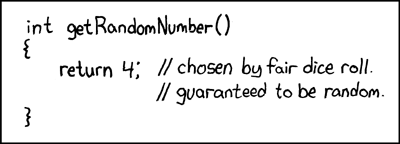
\includegraphics[width=0.4\textwidth]{figures/random_number.png}

  \hspace*{\fill}---Randall Munroe (\href{http://xkcd.com/221/}{XKCD})
\end{figure}
When generating random numbers, you'll want to take care in the methods you use; some RNGs are most definitely better than others.
You can always code your own, but Fortran has a few reasonably good subroutines to do it for you.
The default \texttt{gfortran} installation provides access to a low-level \texttt{\keyword{rand}()} function, but you'll almost certainly want to use the more sophisticated \keyword{random\_number} subroutine instead; it generates much higher quality random numbers and automatically threads over (fills) arrays.
When you've ironed out your algorithm and want to start collecting data, you should also remember to seed the RNG.
Computers generate random numbers by way of a procedural mathematical formula, so using the same seed produces the same series of random values.
The subroutine in \autoref{lst:init_random_seed} will seed the RNG with entropy collected by the system if it's available, otherwise it will use the current time \& process ID.
\lstinputlisting[float=htbp,label=lst:init_random_seed]{examples/init_random_seed.f90}

The Fortran random number generator produces uniformly distributed reals on the interval\footnote{Be careful with operations that might fail with \texttt{0.0d0}.} $\left[0, 1\right)$, but simulations often require numbers drawn from a different distribution. 
For this, we again turn you to \emph{Numerical Recipes}; it describes several methods for generating nonuniform random variates including rejection sampling for gamma, poisson, and binomial distributions and the Box-Muller transform for normal distributions. 

\appendix
\chapter{Linear algebra}
\label{chap:Linear algebra}

When it comes to linear algebra, don't try to write your own routines, always use the BLAS (Basic Linear Algebra Subprograms) and \idx{LAPACK} (Linear Algebra PACKage)\footnote{\url{http://www.netlib.org/lapack/}.
Under Ubuntu, install\index{LAPACK!installation} the \texttt{liblapack-dev} package to obtain BLAS and \idx{LAPACK}, and don't forget to add \texttt{-lblas} and \texttt{-llapack} to \texttt{\$(LIBS)} in your \texttt{Makefile}.} libraries.
Everyone does.
Maple, Mathematica, MATLAB and Python (with NumPy and SciPy) all use it under the hood.
The \texttt{dot\_product} and \texttt{matmul} intrinsics in Fortran are implemented with it.
It's installed on every supercomputer and contains some of the most sophisticated and optimized code known to man.
The fact that these libraries are written in Fortran is actually one of the main reasons to use Fortran for high-performance computing.
Nevertheless, BLAS and \idx{LAPACK} can be a bit low-level sometimes, and the Fortran~77 syntax doesn't help matters much.
For your convenience, we therefore provide two functions for common tasks: calculating the inverse and the eigenvalues + eigenvectors of a real symmetric matrix.
This should help you get started.
For other functions, use Google.
BLAS and \idx{LAPACK} are quite extensively documented.
\lstinputlisting[float=htbp,label=lst:invertMatrix]{examples/invertMatrix.f90}

\lstinputlisting[float=htbp,label=lst:calculateEigensystem]{examples/calculateEigensystem.f90}


\chapter{Plotting with PLplot}
\label{chap:PLplot}

Plotting the results of your calculation from Fortran is easiest with \href{http://plplot.sourceforge.net/}{PLplot}.
PLplot is a cross-platform scientific plotting package with support for multiple programming languages.
Under Ubuntu, you need to install the packages \texttt{libplplot-dev} and \texttt{plplot11-driver-cairo}.
The \texttt{plplot-doc} package might also come in handy.
If you have it installed, you can access the documentation of, \eg, the \texttt{plline} subroutine by typing
\begin{verbatim}
$ man plline
\end{verbatim}
on the command line.

In order to successfully compile a program using PLplot, you need quite a few compiler flags and libraries.
However, most Linux distributions are smart enough to figure that out for you.
Add the following two lines near the top of your \texttt{Makefile}, but after the declarations of \texttt{FFLAGS} and \texttt{LIBS}:
\begin{verbatim}
FFLAGS += $(shell pkg-config --cflags plplotd-f95)
LIBS += $(shell pkg-config --libs plplotd-f95)
\end{verbatim}
The \texttt{pkg-config} command will generate the correct compiler flags on the fly.

\section{Plotting functions}

As a quick introduction to using PLplot, we'll go through \autoref{lst:PLplotDemo} step by step:
\lstinputlisting[label=lst:PLplotDemo]{examples/PLplotDemo.f90}
%\lstinputlisting[caption=PLplotDemo (continued),float=htbp,label=lst:PLplotDemo2,firstline=44,firstnumber=44]{examples/PLplotDemo.f90}
\begin{itemize}
  \item \texttt{\keyword{use} plplot} imports the PLplot functions and subroutines into our program.
  \item \texttt{\keyword{call} plparseopts(PL\_PARSE\_FULL)} parses any command-line arguments of your program that are relevant for PLplot (see below).
  \item By default, PLplot plots all figures on a black background with red axes.
    This is inconvenient, especially for printed figures.
    Lines 11--19 change the color scheme of color map 0 (which is used for line plots) to that of gnuplot (with the exception of color 0, since that's the background color).
  \item All plotting commands must be given between the calls to \texttt{plinit} and \texttt{plend}.
  \item \texttt{plot\_x2} plots the function $y=x^2$ for \texttt{n} values between \texttt{x1} and \texttt{x2}.
  \item The \texttt{linspace} subroutine generates a linearly spaced array, similar to the MATLAB function of the same name.
  \item \texttt{\keyword{call} plcol0(7)} sets the current foreground color to 7 (black), which we use for the axes and labels.
    The call to \texttt{plenv} sets the minimum and maximum values of the axes, scales the plot to fill the screen (the first \texttt{0} parameter) and draws a box with tick marks (the second \texttt{0}).
    \texttt{pllab} is then used to set the $x$ and $y$ labels and the title of the plot.
  \item Finally, we draw a red line (color 1) through the points with \texttt{plline} and draw the points themselves in green (color 2) with \texttt{plpoin}.
    The points are drawn with the `+' glyph (code 2).
\end{itemize}
If the program compiles successfully, you can run it with
\begin{verbatim}
$ ./plplotdemo -dev xcairo
\end{verbatim}
The argument \texttt{-dev xcairo} tells PLplot to use the Cairo X Windows driver, which will open a window showing the plot.
It is also possible to generate a PostScript image by typing
\begin{verbatim}
$ ./plplotdemo -dev pscairo -o demo.ps
\end{verbatim}
and similarly a PDF with \texttt{pdfcairo}. You can find out about the command-line parameters by running
\begin{verbatim}
$ ./plplotdemo -h
\end{verbatim}
or by specifying no arguments at all.

\section{3D animations}

For some programs, such as a molecular dynamics simulation, it is convenient to be able to watch the motion of particles in real time.
For this we'll make use of the 3D plotting facilities of PLplot.
First, we setup the viewport with
\lstinputlisting[lastline=11]{examples/PLplot3D.f90} % Note, these 3 listings all draw from the same source file. Any changes there require a MANUAL reindexing of the firstline and lastline values!
Since the animation will play real-time, we specify the Cairo X Windows driver directly with \texttt{plsdev} instead of parsing the command line.
Lines 7--11 map the world coordinates---bounded by \texttt{xmin}, \texttt{xmax}, \emph{etc.}---to the screen.
This will result in a box which is rotated by 45 degrees around the $z$ and $x$ axes.
We end the program with
\lstinputlisting[firstline=12, lastline=13, firstnumber=12, caption=, nolol]{examples/PLplot3D.f90}
The call to \texttt{plspause} makes sure the program terminates after the animation finishes, instead of leaving the last frame on screen indefinitely.

We plot particles by calling the following subroutine:
\lstinputlisting[firstline=14, firstnumber=14, caption=, nolol]{examples/PLplot3D.f90}
\texttt{xyz} is a $3\times n$ array, with the first row containing the $x$ coordinates of the particles, the second the $y$, and the third the $z$ coordinates.
We first clear the screen with \texttt{plclear}, then draw the axis with \texttt{plbox3}, and finally the particles with \texttt{plpoin3}.
The particles are drawn as small circles (code 4).
Finally, we update the screen by calling \texttt{plflush}.
Calling \texttt{plot\_points} repeatedly results in a smooth animation.
Although this works quite well for checking the movement of particles, PLplot is not a 3D engine and won't run at more than about 100 frames per second.
We therefore recommend not plotting every step in your simulation, but skipping a few frames.
For more documentation on PLplot, Google is your friend.


\chapter[Parallel computing]{Parallel computing: employing a thousand monkeys}
\label{chap:Parallel computing}

\begin{quote}\small
  \emph{``Here be dragons.''}
\end{quote}
If you have a multicore processor, or even multiple processors or machines available, one obvious way to speed up your code is to employ multiprocessing.
However, this is a difficult and dangerous endeavor, especially if you don't have any prior experience.
Parallel programs are far more difficult to write and debug than sequential ones, mostly because concurrency introduces entire classes of potential bugs, like race conditions and deadlocks.
Also, even if it does work, it's not always beneficial.
Some algorithms simply don't scale to multiple processors.
Nevertheless, parallel programming is unavoidable in high-performance computing.
While a true introduction is outside the scope of these notes, we'll give a few guidelines that might help you from accidentally shooting yourself in the foot:
\begin{itemize}
  \item\textbf{Make sure your program works first.} Although this is true for optimizations in general, it is doubly so for parallel programs.
    Programs are much harder to debug when they run in parallel, so leave parallelization for the final step.
  \item\textbf{Check whether the bottleneck in your program benefits from parallelization.} Not every algorithm scales well.
    It would be a waste of time to spend effort parallelizing your code only to discover that it's now actually slower.
  \item\textbf{Use OpenMP.}\footnote{OpenMP is available for C, \Cplusplus and Fortran.
    If you are using \Cplusplus, the \emph{Intel Threading Building Blocks} library is a possible alternative; it has high-level support for certain algorithms and data structures.} For ICCP you won't be using supercomputers or systems with multiple nodes.
    Sophisticated libraries like MPI\footnote{Message Passing Interface: a standardized protocol for communications between nodes in a cluster---used on pretty much every supercomputer in the TOP500.} are overkill and introduce needless complexity.
    OpenMP only works on single machines with shared memory, but it is by far the easiest framework to use.
    All you need to do is add \texttt{-fopenmp} to \texttt{FFLAGS} and \texttt{LDFLAGS} in your \texttt{Makefile} and add a few directives to your code.
    For example
\begin{lstlisting}[caption=, nolol]
  !$omp parallel do
  do i = 1, n
      y(i) = x(i) * i
  end do
  !$omp end parallel do
\end{lstlisting}
    will execute the loop in parallel. Use Google for more information on how to use OpenMP.
  \item\textbf{Don't use more threads than you have physical cores.} This may seem like stating the obvious, but it actually happens rather often.
  Most modern Intel processors implement hyper-threading.
  This doubles the apparent number of cores, which helps with task switching when you're running many different programs at once.
  However, for CPU intensive calculations, like the ones you'll be running, the threads will be competing for the available physical cores.
  In that case doubling the number of threads will actually harm performance.
\end{itemize}


\chapter{Revision control}
\label{chap:Revision control}

\begin{quote}
\emph{``And then there's \texttt{git rebase --interactive}, which is a bit like \texttt{git commit --amend} hopped up on acid and holding a chainsaw---completely insane and quite dangerous but capable of exposing entirely new states of mind."} \\ \hspace*{\fill}---Ryan Tomayko
\end{quote}

A revision control system is perhaps the third most useful tool to a programmer after only the editor and compiler.
The idea is simple: you give a piece of software a description of recent changes you've made to your code, and that software will efficiently log the changes and description for you to view and optionally undo should you need to.
Written by Linus Torvalds and popularized by websites like \href{https://Github.com/}{Github}\index{Git!Github}, Git\index{Git|(} is probably the most widely used revision system around.
While a a full Git tutorial is far beyond the scope of this introduction, knowledge of a few basic commands can potentially save you a ton of time (and headaches!) down the road.

To get started, you'll want to install the \texttt{git}, \texttt{gitk}, and \texttt{git-gui} packages on Ubuntu. Next, let's assume you've created an \texttt{iccp/} directory with one file, \texttt{myProg.f90}, that already has some content. Navigate to the \texttt{iccp/} directory and type
\begin{verbatim}
$ git init
$ git add .
$ git commit -m ``Initial commit''
\end{verbatim}
This does a few things for you:
\begin{itemize}
  \item \texttt{git init} creates a git repository of \texttt{iccp/} by placing the current directory (and all sub-directories) under revision control.
    Any files and directories that get added to \texttt{iccp/} can be tracked as part of the current project.
  \item \texttt{git add .} adds every file's local changes to the \emph{staging area} or \emph{index}.
    The index tracks changes for you to inspect before they become an official part of the project history.
  \item \texttt{git commit -m ``Initial commit''} takes everything in the index and adds it to the history with the description ``Initial commit''.
\end{itemize}
You can add future changes in \texttt{myProg.f90} to the history in a similar way:
\begin{lstlisting}[style=prompt, nolol, linewidth=30cm]
  $ git add myProg.f90            # or . to add everything under ./
  $ git commit -m "Fixed bug XYZ" # use a msg appropriate for your changes
\end{lstlisting}
Similarly, you can check the current status of the index with \texttt{git status}. 
The output will display changes both staged and not staged in the index for the next commit, allowing you to tweak things as necessary.

If, after some bleary-eyed, hungover coding, you realize you've made a horrible mistake since your last commit, you can check a file's current state against the most recent history with
\begin{verbatim}
$ git diff <file>
\end{verbatim}
And to delete any changes you've made
\begin{verbatim}
$ git checkout <file>
\end{verbatim}
You can view the entire project history with the \texttt{gitk} program, including file diffs, commit messages, and authors. Similarly, \texttt{git gui} provides a handy interface for staging commits. You can write/amend commit messages, see which files have changed and what files you've added to the index, push/pull to remote repositories, etc.

There are only a handful of ways to completely delete data from the repository once you've committed it\marginnote{It's a good idea to avoid the more dangerous commands like \texttt{git rebase} and \texttt{git gc} that \emph{can} permanently remove things from the project history. \textcolor{red}{\emph{Always}} think about commands before you run them!}, so unless you're \emph{really} trying to rewrite history your code is reasonably safe from git-mishaps.
That said, here are some tried and true tips to make the most of Git:
\begin{itemize}
  \item \textbf{Commit frequently}. The more commits you have, the more the history can help you.
    If you're trying to find a problem introduced in a new subroutine, it's much easier to search through ten lines of code you added in the past half hour than the 200 lines you added since Monday.
  \item \textbf{Commit \emph{logically}}. Commit complete logical units (like writing a function, fixing a bug, or formatting output) instead of just ``at the end of the day.''
    This greatly helps in reasoning about the development of your code---and thus undoing problems!
  \item \textbf{Use descriptive commit messages}. Messages like ``Fixed bug in force calculation'' and ``Implemented averaging function'' work far better than an endless series of ``nightly backup''s.
    If you can't easily reason about what's changed in your code, tracking the changes will do very little to help you.
\begin{marginfigure}[-1.1cm]
  \centering
  \label{fig:git_commit}
  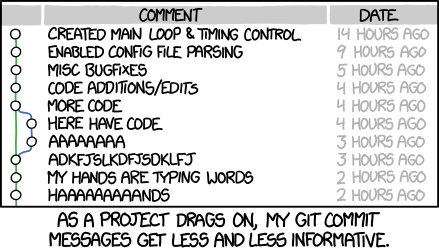
\includegraphics[width=\textwidth]{figures/git_commit.png}

  \hspace*{\fill}---Randall Munroe (\href{https://xkcd.com/1296/}{XKCD})
\end{marginfigure}
  \item \textbf{Commit the bare minimum}. Only commit what's needed to recompile a functional program.
    Git just tracks the differences in files between commits to save space, but executables, output data, PDFs, images, etc. all require a totally new copy in the history every time they change (and that's frequently!)
    Tracking a \texttt{.gitignore} file with some simple patterns can automatically ignore files of a similar type.
  \item \textbf{Learn the advanced Git features}. Basic commits barely scratch the surface of Git's functionality.
    Branching lets you test drive changes in a copy of your code in an easily-reset sandbox, the network features let you not only backup code but also collaborate with other developers, and \texttt{git-bisect} can help you \emph{automatically} pinpoint exactly where and when a bug crept in.
\end{itemize}

You can find all of the example codes given in these notes at the \href{https://Github.com/ICCP/coding-notes}{ICCP/coding-notes repository} on Github.
To use them, you'll want to \texttt{clone}\footnote{A clone is a complete local backup of the repository. It contains the entire project history and may itself be cloned and pulled from.} the repository with
\begin{verbatim}
$ git clone git@github.com:ICCP/coding-notes.git
\end{verbatim}
You can then download any future changes to the repository with a \texttt{git pull} command inside the libICCP directory

Because of Git's popularity, the internet has a number of fantastic resources for learning to use it. 
\href{http://learn.Github.com/p/index.html}{Github Learning}, \href{http://git-scm.com/book}{Pro Git}, \href{http://think-like-a-git.net/}{Think Like a Git}, and \href{http://gitready.com/}{Git Ready} all offer very good tutorials and explanations.
And for the truly enthusiastic, \href{http://pcottle.github.io/learnGitBranching/}{LearnGitBranching} gives an interactive git session complete with tasks designed to simulate common git operations.\index{Git|)}

\backmatter
\Chapter{Further reading}{a.k.a\ programmer humor}
\begin{itemize}
  \item \href{http://www.pbm.com/~lindahl/real.programmers.html}{Real programmers don't use Pascal} (\textbf{Mandatory})
  \item \href{https://gist.github.com/alanbriolat/3135713#file-fortran_hell-f95}{The many faces of function definition in Fortran 95} (\textbf{Mandatory})
  \item \href{http://www.codinghorror.com/blog/2006/05/the-ten-commandments-of-egoless-programming.html}{The Ten Commandments of Egoless Programming}
  \item \href{http://james-iry.blogspot.com/2009/05/brief-incomplete-and-mostly-wrong.html}{A Brief, Incomplete, and Mostly Wrong History of Programming}
  \item \href{https://www.gnu.org/fun/jokes/ed-msg.html}{\texttt{Ed, man! !man ed}}
  \item \href{http://blog.sanctum.geek.nz/vim-koans/}{Vim koans}
\end{itemize}

\end{document}
